In this Section we will describe all the techniques used for cleaning and preparing the data for the learning phase.

%-------
\subsection{Data Cleaning}

Since the NSL-KDD dataset is already an enhanced version of the older KDD '99 CUP dataset, little additional cleaning had to be performed: the set had already been cleaned from redundant data and null values \cite{nslkdd}. Also, the ratio between normal and anomalous entries is good for machine learning purposes.

The only step taken at this stage, a part from loading the \texttt{.arff} files and decoding strings using UTF-8, was to change all the entries with \textit{http\_XXX} as their  \texttt{service} values into \textit{http}, where \textit{XXX} denotes the port number.

This decision was taken since the port of an http connection, which is specified in the protocol string only for some entries, is very unlike to be correlated with an anomalous behaviour in a general case. Also, leaving this distinction could lead to new http connections on previously unseen ports to not be recognized correctly by the algorithm.

This cleaning has later been proven to be an effective solution for partially reducing overfitting.

%-------
\subsection{Categorical Columns Encoding}

After cleaning the dataset, the second step was to convert all categorical columns into one-hot encoded columns. This means that, for each distinct value of each categorical column, a new column is generated, contaning '1' for the rows belong to that category and '0' elsewhere.

This kind of encoding is the most popular choice when it comes to preparing data for ANN learning \cite{encoding}. This is done to prevent the algorithm from interpreting categories as numbers, which can lead to problems like the algorithm considering a category the mean of other two categories etc.

The affected columns in particular are:

\begin{itemize}
    \item service
    \item protocol\_type
    \item su\_attempted
    \item flag
    \item class (target variable)
\end{itemize}

The dataset resulting from this encoding contains \textbf{124} columns, of which 2 are the target columns.

Note that, a part from the target column, all other binary columns where not affected by the encoding. This is to avoid redundant columns, since binary features would have two corresponding encoded columns in which one can be directly inferred by observing the other.

%-------
\subsection{Normalization}
\label{subsec:norm}

Having encoded the categorical columns, now the numerical columns have to be treated. In particular, it was decided to apply MinMax \cite{minmax} normalization to both discrete and continuous columns. The normalization process has been accomplished as follows: 

\begin{itemize}
    \item Fit the model onto the train set
    \item Transform the train set
    \item Transform the test set (with the same normalization model)
\end{itemize}

Figure~\ref{fig:trainnorm} describes the distribution of the numerical values in the train set after normalization, while Figure~\ref{fig:testnorm} illustrates the same transformation applied to the test set. As we can see, all values in the train set are correctly normalized between 1 and 0, while the test set contains some values that are greater than the maximum found on the train set, hence their normalized values is greater than 1.


\begin{figure}[h]
    \centering
    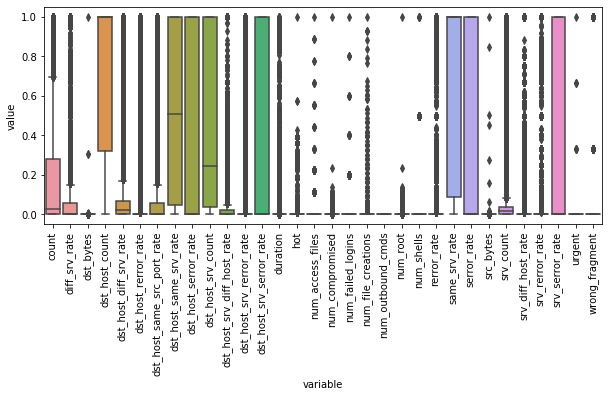
\includegraphics[width=\linewidth]{img/box_train.png}
    \caption{Distribution of numerical values in the normalized train set.}
    \label{fig:trainnorm}
\end{figure}


\begin{figure}[h]
    \centering
    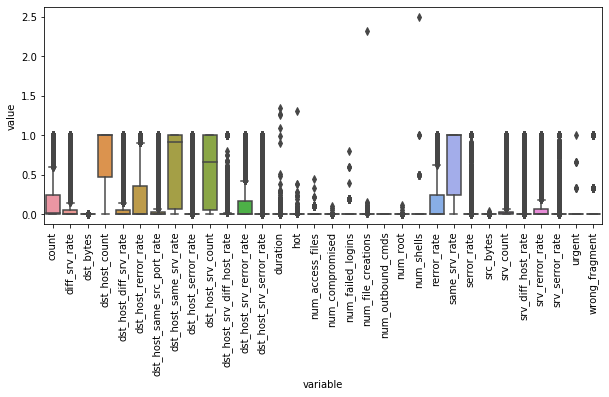
\includegraphics[width=\linewidth]{img/box_test.png}
    \caption{Distribution of numerical values in the normalized test set.}
    \label{fig:testnorm}
\end{figure}

\FloatBarrier